\subsection{Sensing Subsystem}
\label{sec:sensing_subsystem}

\begin{figure}[H]
    \caption{Sensing subsystem block diagram}
    \centering
    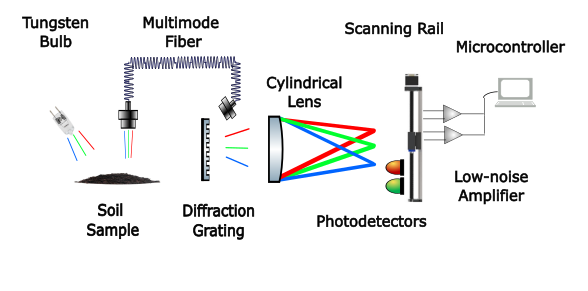
\includegraphics[width=0.75\textwidth]{images/Schematic Diagram 2.png}
\end{figure}

\paragraph{Overview} The system determined what automation was needed to optimize the gardening environment using a Near Infrared Optical Spectrometer. The spectrometer probed the soil with a broad band light source, exciting electromagnetic waves in the weak bonds of the material. These waves were collimated into a fiber optic cable and transmitted into a closed chamber. The beam was guided into the housing and reflected off a diffraction grating, which separated wavelengths by angle. A focusing lens positioned the separated spectrum on a surface several inches away. Then Visible and Near Infrared optical sensors were scanned across the surface. At every position, the system microcontroller recorded the sensor positions and amplitudes. The data determined what actions the system would take, whether mechanically or via messaging.

\begin{figure}[H]
    \caption{Light Collection System}
    \centering
    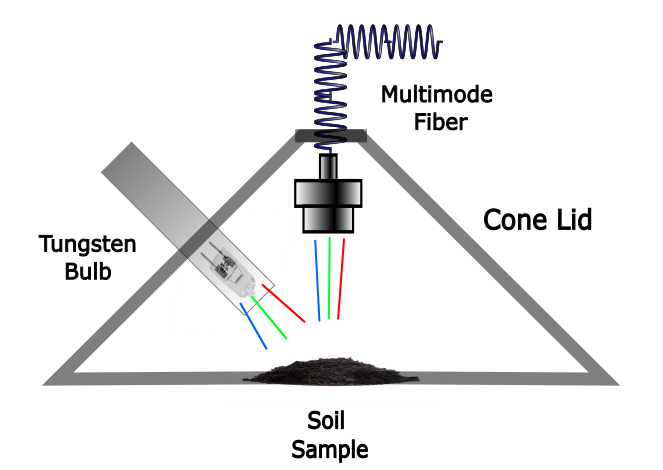
\includegraphics[width=0.25\textwidth]{images/Light Collection.png}
\end{figure}

\subsubsection{Light Collection} The light from the bulb shone on a patch of soil and reflected onto the fiber head collimator. In order to maximize the effect of reflectance on the sample, the bulb was seated in a reflective metal tube which shielded reflections from entering the fiber head.

\begin{figure}[H]
    \caption{Spectral Output of a Tungsten Lamp}
    \centering
    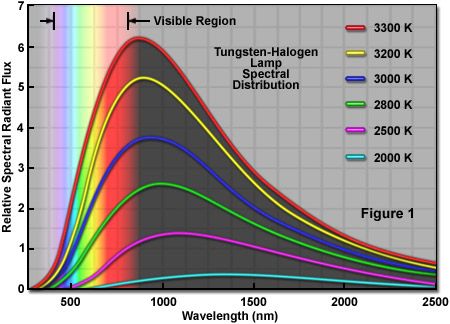
\includegraphics[width=0.75\textwidth]{images/TungstenLamp.jpg}
\end{figure}

\subsubsection{Light Source} The spectrum of interest was from 400nm to 1700nm, however, not all data points were necessary for the system decision matrix. This initially suggested the use of LED lights as a cheap, low power solution, but the number, target wavelengths, and spectral widths of LEDs created several challenges. Broad band Super Luminescent Diodes dramatically reduced the complexity of the problem, but they were an emerging technology with high material cost, placing even the cheapest devices orders of magnitude outside of the project budget. Thankfully, the desired effect could be achieved with a tungsten lamp. Tungsten was a material which emitted a broad range of frequencies, covering the spectrum of interest and then some.
\paragraph{Soil Conditions} The optical signal emitted by the soil was weak, so it was essential that the spectrometer was influenced as much as possible by the content of the soil and as little as possible by the topology of the surface. A well-mixed, smoothly flattened, gently compressed soil sample provided the best conditions for constructing a spectrograph. If there were ridges or depressions along the sample, too much or too little optical signal would pass into the spectrometer, creating an apparent signal strength for wavelengths that was not representative of the soil emission. There were several ways to control these conditions. One was to require the user to retrieve a sample for each scan and deposit it into a spectrometer bay. Another was to require the user to flatten the soil with a spatula or other implement and position the scanner input near the soil. These reduced ease of use, which was a target for the project. Another issue was that the position of the signal input and the tungsten light source relative to the soil sample had to be consistent to avoid signal error, for the same reasons as above. In one study\cite[]{Mouazen2007}, this issue was resolved by building a transparent block with slots to hold the light source and the input beam. Their design was represented below, showing the block attached at the rear of a plow chisel for clearing soil while scanning. We solved the problem of soil topology and light position the same way, by mounting the light source and input fiber in a block of some transparent material like acrylic.

\begin{figure}[H]
    \caption{Coupling a diffuse light into a fiber}
    \centering
    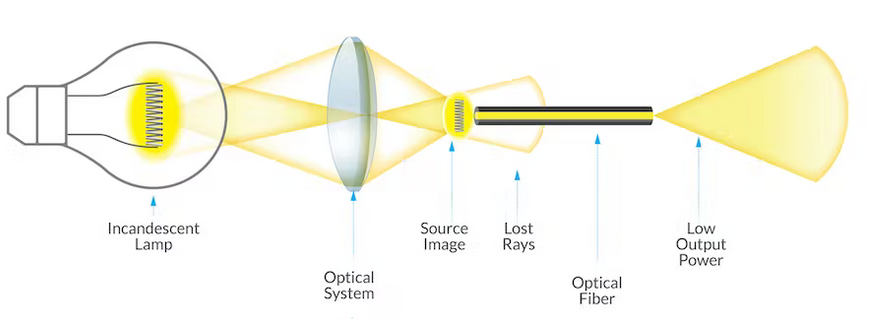
\includegraphics[width=0.75\textwidth]{images/CouplingDiffuseLighttoFiber.png}
\end{figure}

\paragraph{Fiber Optics} Fiber optic cables were a standard input for spectrometer devices since they allowed nearly unlimited flexibility for the position and orientation of the target area relative to the device. The basic ray trace for a lens coupling light into a fiber was shown below. Fiber cores faced some basic limitations when it came to coupling. The maximum possible coupling efficiency could be achieved by pressing the optical surface of the fiber core up against a light source with equal random output in every direction (reference). If the fiber was moved some distance away from the source, less light would impede on the core-air interface. If the core diameter was increased, this would increase the light incident on the core. Light moving in random directions would also strike the fiber core at various angles, however, not all angles of incidence would couple into the fiber. Only rays within the numerical aperture of the fiber were accepted. This was why installing large lenses at the end of the fiber did not increase the maximum possible amount of light that could be coupled. The maximum angle was determined by the fiber, rather than the collimator.

This project involved a large diffuse source, the illumined soil. The Fiber collimator was attached to the fiber cable via their SMA connectors, and then the collimator was set in an acrylic block so that it rested 8.06mm above the soil. The block also had a slot for the Light source to illuminate the soil at an angle, similar to the arrangement of the source and sensor in a computer mouse above a mousepad.

The signal traveled through the fiber and up into the spectrometer housing, where the other connector of the cable was mounted in place. Another collimator took the output beam and collimated it so that it propagated through free space into the housing. The collimator had an output beam diameter of 1.7mm. This planar wavefront struck the diffraction grating.

\begin{figure}[H]
    \caption{Grating Angular Calculation}
    \centering
    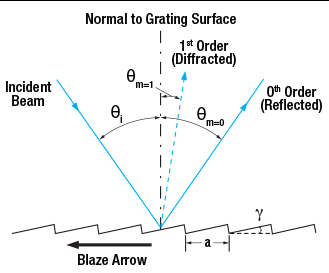
\includegraphics[width=0.4\textwidth]{images/ThorlabsGratingTutorial.png}
\end{figure}

\subsubsection{Diffraction Grating} The reflective diffraction grating was a glass mirror with a thin layer of metal deposited on the surface. 1200 lines per millimeter were scored out of the metal horizontally. When a planar wavefront hit the surface of the grating, it reflected off. The confinement of the wave on the surface of the material induced a change of direction proportional to the frequency of the beam, separate from the direction of reflection, equal to the angle of incidence from normal. In order to direct the diffracted beam away from the incoming beam, the grating was placed at an angle of 45 degrees. This changed the angle of incidence and determined the angular range of the system. To increase the working range of the grating, the lines scored into it were blazed at an angle so that light approaching the surface from the angle struck the scored metal at zero degrees from normal. The angular spread of the system ranged from the lower angular wavelengths around 400nm up to 1700nm and beyond.

\begin{equation}
    a[sin(\theta m)+sin(\theta i)] = m\lambda
\end{equation}

\begin{figure}[H]
    \caption{Diffraction angle calculation}
    \centering
    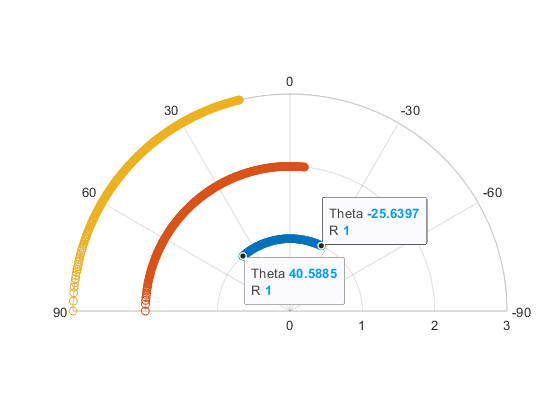
\includegraphics[width=0.75\textwidth]{images/PolarPlot.png}
\end{figure}

This meant that the spread of the diffracted light was 38 degrees in and 21 degrees out from both the near edge and the far edge of the collimated beam on the surface of the grating. In order to capture this light and sort it so that the scanner could proceed linearly through each band, a focusing optic was needed that covered the full angular range.

\begin{figure}[H]
    \caption{Ray Trace of Diffraction Grating}
    \centering
    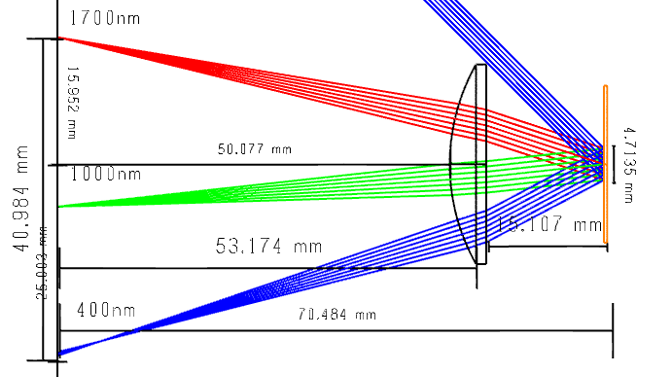
\includegraphics[width=0.75\textwidth]{images/RayTrace.png}
\end{figure}

The beam coming out of the fiber had a nonzero width. When the 1.7mm diameter beam hit the surface of the grating, since the grating was at 45 degrees from the beam, light was propagating from an area with a diameter larger than 1.7mm.

\subsubsection{Focusing Lens} The diffraction grating diverged the beam away from the sensor surface. This divergence could be corrected with a lens, focusing the divergent light to a spot the size of the sensor or smaller. There were two lens designs that could work, spherical and cylindrical. Spherical lenses were polished with a radius of curvature along both the horizontal and vertical axes. The advantage of a spherical lens was that they were generally cheaper to manufacture and available in a wider variety of sizes and shapes. The spot size of a circular beam passing through a spherical lens was determined by the distance from the focal length, and the spot was circular.

Cylindrical lenses were cut with a radius of curvature along the horizontal axis, but flat along the vertical axis. A circular beam that passed through a cylindrical lens was focused to the shape of an ellipse, allowing for more vertical flexibility of alignment. Plano-cylindrical lenses offered another advantage; they had a flat bottom, perpendicular to their planar back. This meant they could be stood upright and pressed against a flat surface, dramatically reducing the complexity of the optical mount required to hold them in place.

The dimensions and position of the lens were determined by two things, the angular range of the spatially separated beams coming off the reflective diffraction plate, and the width of the scanning region. The lens was also constrained by the angle and width of the input beam, as shown in the ray trace below. If the width of the lens came within a few wavelengths of the beam approaching the diffraction plate, the beam would diffract around its edge.

\begin{figure}[H]
    \caption{Spot Diagram}
    \centering
    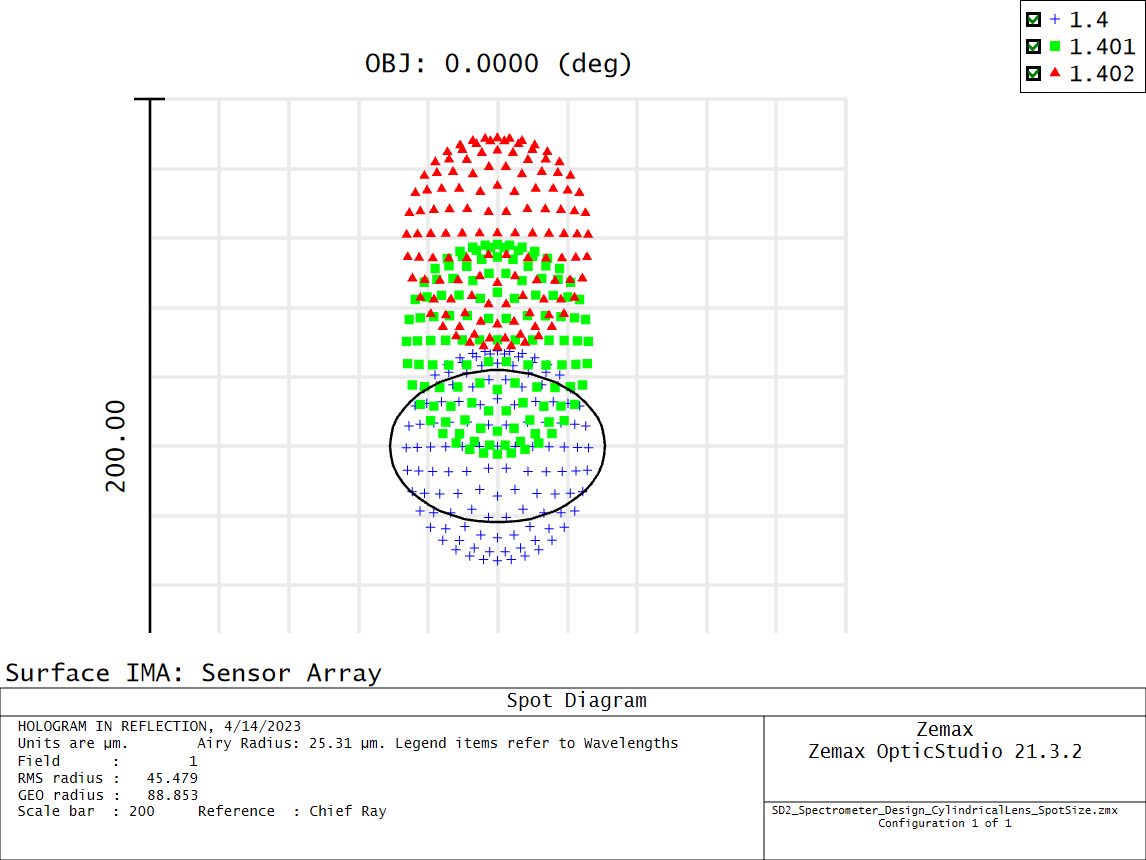
\includegraphics[width=0.75\textwidth]{images/SpotDiagram.png}
\end{figure}

The spot size of an idealized raytrace yielded 27$\mu$m, with ~30$\mu$m between spot centers. This was excellent, since the airy disk suggested by the ray trace was within an order of magnitude. This meant the arrangement of the components did not raise the lower limit of the spectral resolution above 2nm, although it was doubtful the nonideal system would achieve such precision.

\begin{figure}[H]
    \caption{Sensing Schematic}
    \centering
    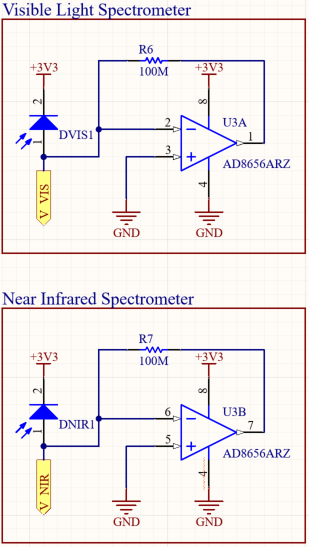
\includegraphics[scale=1.5]{images/SensorSchematics.PNG}
    \label{fig:sensor-schem}
\end{figure}

\subsubsection{Circuitry} The Photodiode worked by converting a small portion of the incident light into electrical current across the face of the semiconductor. There were three components to the sensing circuitry. First, there was a voltage divider. This voltage divider provided a clean and stable 1.65V to the anode of the photodiode. The photodiode was reversed bias to create a current when detecting light. From there the second part of the circuit began which was a current-to-voltage converter. The photodiode emitted a current based on the power of light that hit the surface per the area that it hit. Using a 100 M$\Omega$ resistor converted current to voltage at a rate of 1 pA to 100 $\mu$V. There were two issues with this however, first the ADC only had 12-bits and as discussed in the controller section, this resulted in about half a milli-Volt per step. This meant that the system lost about 4x the resolution of the sensor. This is where the last part, the instrumentation amplifier took effect. The instrumentation amplifier took the difference between the voltage output and a reference voltage and scaled all the parts. For example, if the output voltage of the current-to-voltage converter was .3V (which happened to be the dark current of the visible light sensor) subtracting the voltage of the dark current and scaling the remainder helped.

\begin{figure}[H]
    \caption{Soil Spectrograph}
    \centering
    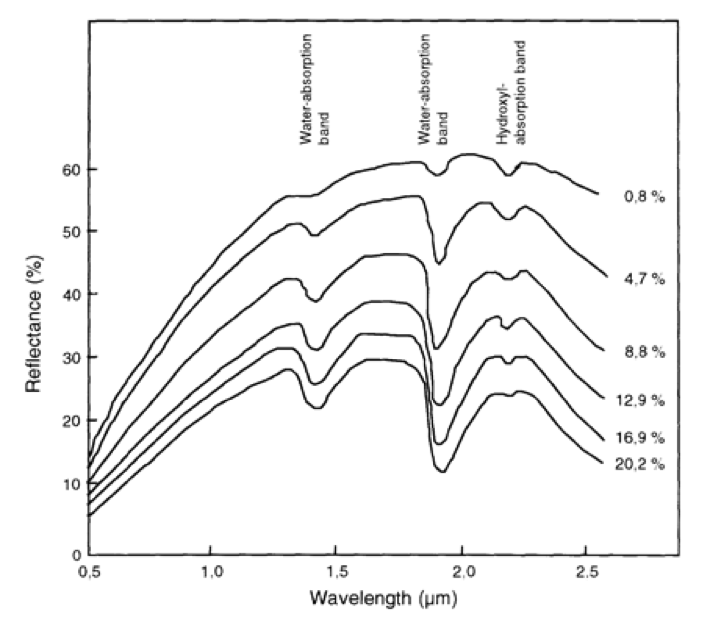
\includegraphics[scale=0.5]{images/GenericSoilSpectra.png}
\end{figure}

\paragraph{Spectrum of Interest} Soil is a heterogeneous combination of organic and inorganic substances, and the balance of soil nutrients contributes directly to the quality of the garden environment. Each substance contributes to the total radiative emission of the soil, so by measuring the traces in a sample with unknown quantities and comparing it to traces from a sample with known quantities, the nutrients can be estimated. Soil Carbon content, Moisture Content, Phosphorous, and pH can all be detected through reflectance within the 400nm to 1700nm range \cite{Mouazen2007}. The spectrograph looked something like the one above.